% This textfile includes
% 3. Analysis procedures
%    ..
%    ..
%    3.4 Pile-up
%    3.5 Event and Object selection
%    3.6 Data and MC comparison
%    3.7 Background estimation
%    3.8 Signal yields

\section{Pile-up reweighting}
At the typical luminosity provided by the LHC, it is common to reconstruct more than one vertex per event. The main event vertex is defined as the one with the highest sum of the $p_{T}^{2}$ of the associated tracks. The presence of additional interactions, known as pile-up (PU). 

The simulation generates the pile-up roughly to match the condition in data, however there are still difference between the pile-up numbers in data and MC. It is neccesary to reweight pile-up distribtuions of MC samples to match the data more precisely. By applying a proper weight to each MC event according to the pile-up distribution from data, the MC samples can describe the data better. Fig.~\ref{fig:PUreweight} shows the number of vertices after pile-up reweighting in both two lepton channel.

\begin{figure}[hbtp]
  \centering
  \subfigure[Number of vertices in muon channel]{
    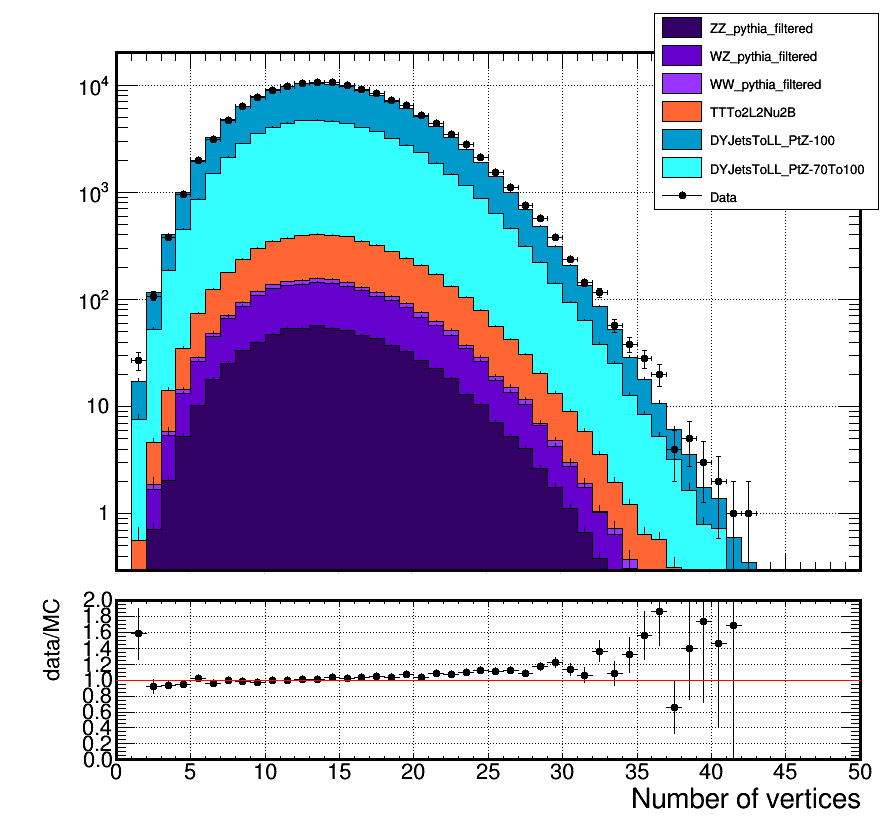
\includegraphics[scale=0.22]{figure/CH3/h_nVtx_Mu.png}}
  \hspace{0.5cm}
  \subfigure[Number of vertices in electron channel]{
    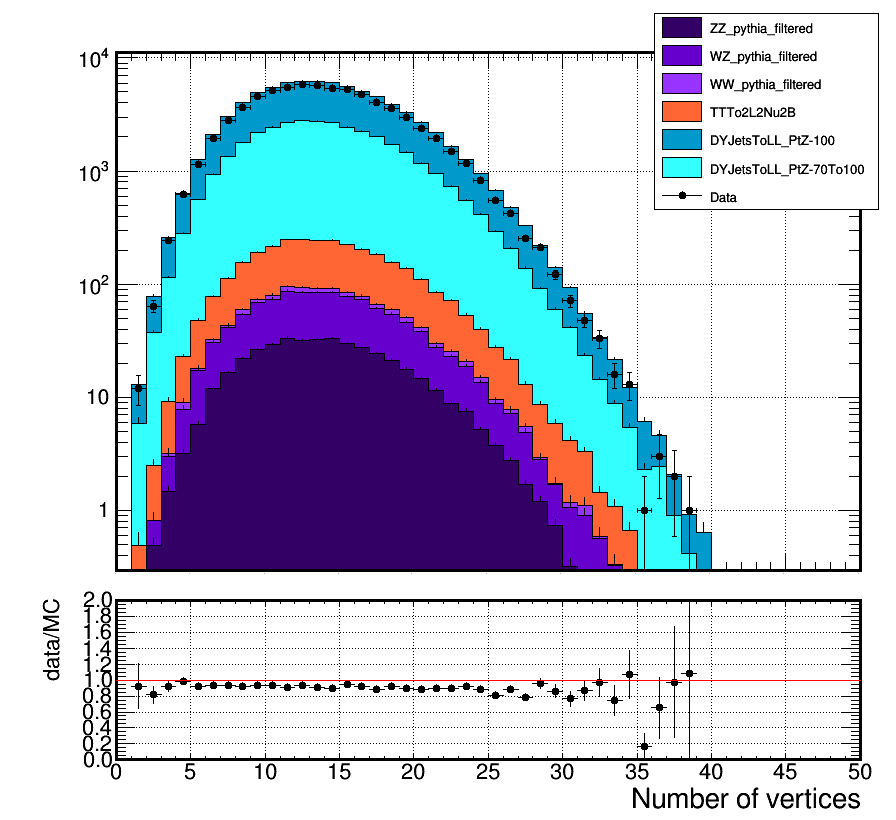
\includegraphics[scale=0.22]{figure/CH3/h_nVtx_El.png}}
  \caption{\label{fig:PUreweight}Number of vertices distributions after pile-up reweighting. Data are compared to the combination of all MC background samples. After reweighting, the distributions are almost identical to the data in both channels.}
\end{figure}



\newpage
\section{Event and Object selection}


\subsection{Lepton Requirements}

\subsection*{Muon Selection}

Besides the muon ID criteria disscussed in section 3.3.1 (Table~\ref{tab:MuonIDtable}), we also require kinematic cuts on the muon candidates. We require that the transverse momentum of the leading muon candidate must be greater than 40 GeV, while the second leading muon transverse momentum minimum threshold is 20 GeV. All muon candidates must be in the psuedo-rapidity region of $|\eta| < 2.4$.

\subsection*{Electron Selection}
Kinematic cuts on the electron candidates are also applied. Although the electron ID selection (Table~\ref{tab:EleIDtable}) already required the pseudo-rapidity of electron supercluster, we cut on the $|\eta| < 2.5$ for electron candidates and all electrons must be outside of [1.4442,1.566] in the $\eta$ region to avoid the ECAL gap. The $p_{T}$ requirement is a bit different from the muon case. Since the HLT trigger already selects electron $p_{T}$ greater than 33 GeV, we require both leading and sub-leading electrons $p_{T}$ greater than 40 GeV in advance.

\subsection{Jet Requirement}
CA8jets in our signal process originate from Higgs decay. If the $Z'$ mass is large enough, the Higgs will be boosted. Therefore we require higher kinematic thresholds to the CA8jets. In every event, there must be at least one CA8jet with $p_{T} > 80$ GeV, $|\eta| < 2.4$, passing loose jet ID and the pruned-jet mass must be greater than 40 GeV to remove jets from backgrounds.

Futhermore, in order to veto leptons that are mis-identified as jets, leptons overlap with jets are removed by the $\Delta R$ cut, i.e. if there's a lepton passing all lepton selections and the spatial distance to a CA8jet smaller than 0.1 ($\Delta R_{jet,lepton} < 0.1$), then the jet will be removed.

\subsection{Z boson Requirement}
The Z boson candidate is reconstructed by adding four-momentum of the selected lepton pair. The Z boson mass is about 91 GeV, therefore we require the reconstructed invariant mass of the Z boson in the mass region [70 GeV, 110 GeV] where is $\pm 20$ GeV to its theoretical mass.

For the CA8jet from Higgs, we require a minimum $p_{T}$ threshold of 80 GeV. Since the transverse momentum of $Z'$ is zero and the mass diffence between Z and Higgs is negligible ($1\textup{ TeV} >> 125 \textup{ GeV} \sim 91 \textup{ GeV}$), the Z and the Higgs boson are back to back at the transverse plane and their $p_{T}$'s are identical. Therefore we require the same minimum $p_{T}$ theshold to the Z boson. Fig.~\ref{fig:genZHPt} shows the transverse momentum distributions from the signal samples.

\begin{figure}[hbtp]
  \centering
  \subfigure[generator level Higgs $p_{T}$ distribustion]{
    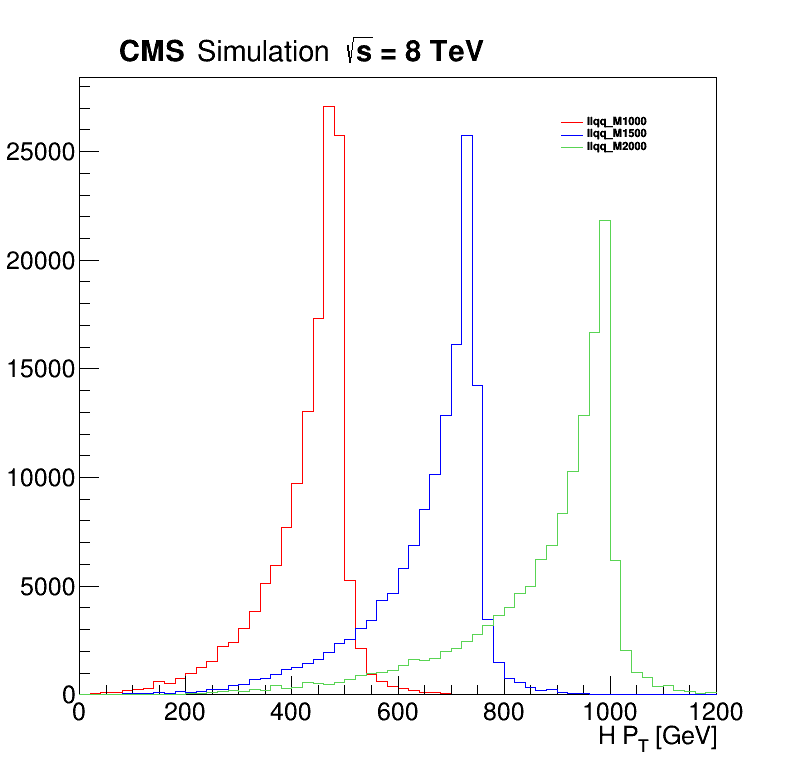
\includegraphics[scale=0.25]{figure/CH3/h_genHPt.png}}
  \hspace{0.5cm}
  \subfigure[generator level Z boson $p_{T}$ distribustion]{
    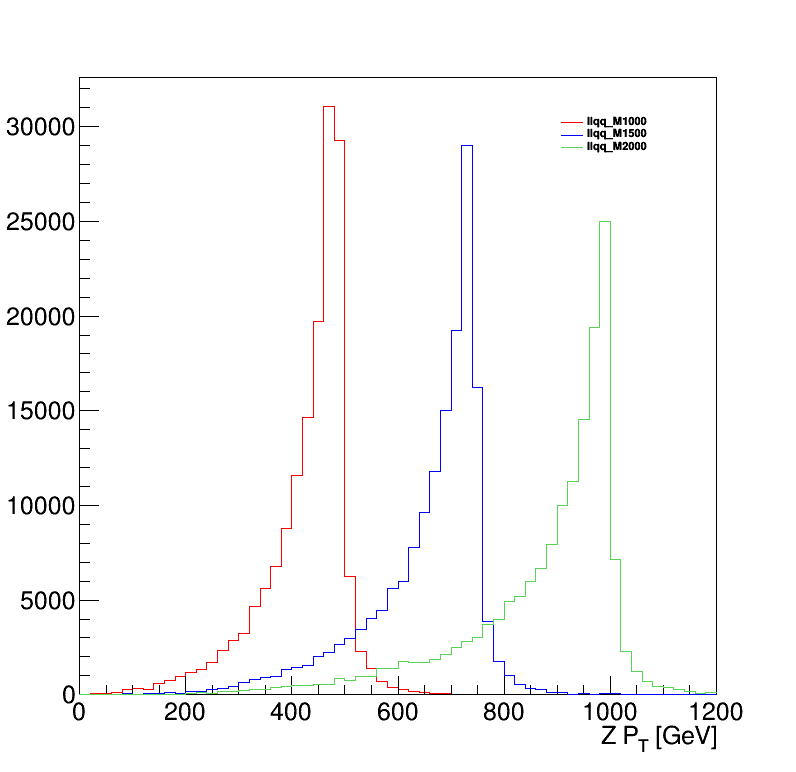
\includegraphics[scale=0.25]{figure/CH3/h_genZPt.png}}
  \caption{\label{fig:genZHPt}Z and Higgs $p_{T}$ distribution are almost identical. We pick three samples with different mass points of $Z'$, 1000 GeV (red), 1500 GeV (blue) and 2000 GeV (green). These plots are made from the generator level signal samples without any proper selections.}
\end{figure}

Finally, all selection requirements are summarized in Table~\ref{tab:preselection}.
\newpage

\begin{center}
  \begin{table}[h]
    \begin{center}
      \begin{tabular}{|lcc|}
        \hline
        \textbf{Selection} & \textbf{Value} & \textbf{Comments} \\ \hline
        Trigger & HLT\_Mu22\_TkMu8 & DoubleMu dataset \\
        & HLT\_DoubleEle33 & DoublePhoton dataset \\ \hline
        Leading muon $p_{T}$ & $p_{T} > 40$ GeV &\\
        Sub-leading muon $p_{T}$ & $p_{T} > 20$ GeV &\\
        Muon $\eta$ & $|\eta| < 2.4$ &\\
        Muon ID & High $p_{T}$ tracker based &\\
        Muon isolation $I_{trk}^{mod}$ & $< 0.1$ &\\ \hline
        Leading electron $p_{T}$ & $p_{T} > 40$ GeV &\\
        Sub-leading electron $p_{T}$ & $p_{T} > 40$ GeV &\\
        Electron $\eta$ & $|\eta| < 2.5$ &\\
        & out of [1.4442,1.566] & To avoid ECAL gap. \\
        Electron ID & HEEP modified &\\
        Electron isolation  & &\\
        $I_{trk}^{mod}$ & $<$ 5 GeV &\\
        $I_{ECAL,HCAL}^{mod}$ & $<$ 2 GeV + 0.03$E_{T}$ & Barrel \\
        & $< 2.5$ GeV & for $E_{T} < 50$ GeV candidates in Endcap\\
        & $< 2.5$ GeV + 0.03$E_{T}$ & for $E_{T} > 50$ GeV candidates in Endcap\\ \hline
        Jet ID & Loose working point &\\
        Jet $p_{T}$ & $p_{T} > 80$ GeV &\\
        Jet $\eta$ & $|\eta| < 2.4$ &\\
        Prunedjet mass & $> 40$ GeV &\\
        Veto jet-lepton overlap & $\Delta R_{jet,lepton} < 0.1$ & Remove the jet satisfies this requirement.\\ \hline
        Z $p_{T}$ & $p_{T} > 80$ GeV &\\
        Z mass window cut & $70 \textup{ GeV} < m_{Z} < 110 \textup{ GeV}$ &\\
        \hline
      \end{tabular}
    \end{center}
    \caption{\label{tab:preselection}Event and object selection requirements used in the analysis.}
  \end{table}
\end{center}

\newpage
\section{Data-MC comparison}

In this section, a comparison between data and simulation is reported for various kinematic observables. It can be seen that the dominant background contribution comes from the Z+jets production, while sub-leading contributions are from $t\bar{t}$ and dibosons can be negligible.

On top of the selections described in previous section, additional regions are defined as following:

\begin{itemize}
\item \textbf{Signal region (SR)}: Represents the phase space where the signal is expected, defined by the prunedjet mass in $110 \textup{ GeV} < m_{prunedjet} < 140 \textup{ GeV}$ region. The range is chosen by $\pm$15 GeV to the mass of Higgs.
\item \textbf{Sidebands (SB)}: Defined by the interval between $70 \textup{ GeV} < m_{prunedjet} < 110 \textup{ GeV}$. This region is signal-depleted. In our case, we don't consider prunedjet mass higher than 140 GeV, because of the poor statistics and the excessive contribution of $t\bar{t}$ events.
\end{itemize}

In the following plots, the data-MC comparison is performed in SB region and all background samples are weighted to the same luminosity as data. The results combined both muon and electron channels. Because of the signal region in data is considered \textbf{blind} in this analysis stage, so they are not shown.

\begin{figure}[hbtp]
  \centering
  \subfigure[Muon energy fraction]{
    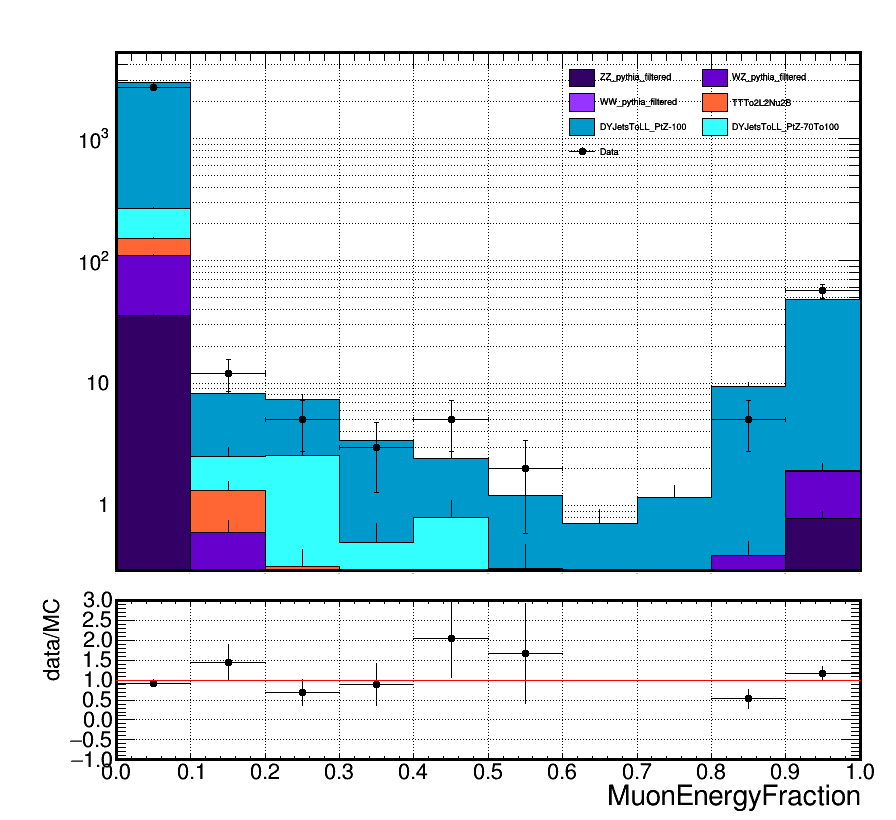
\includegraphics[scale=0.22]{figure/CH3/JetID/h_CA8jetMuEF.png}}
  \hspace{0.5cm}
  \subfigure[Photon energy fraction]{
    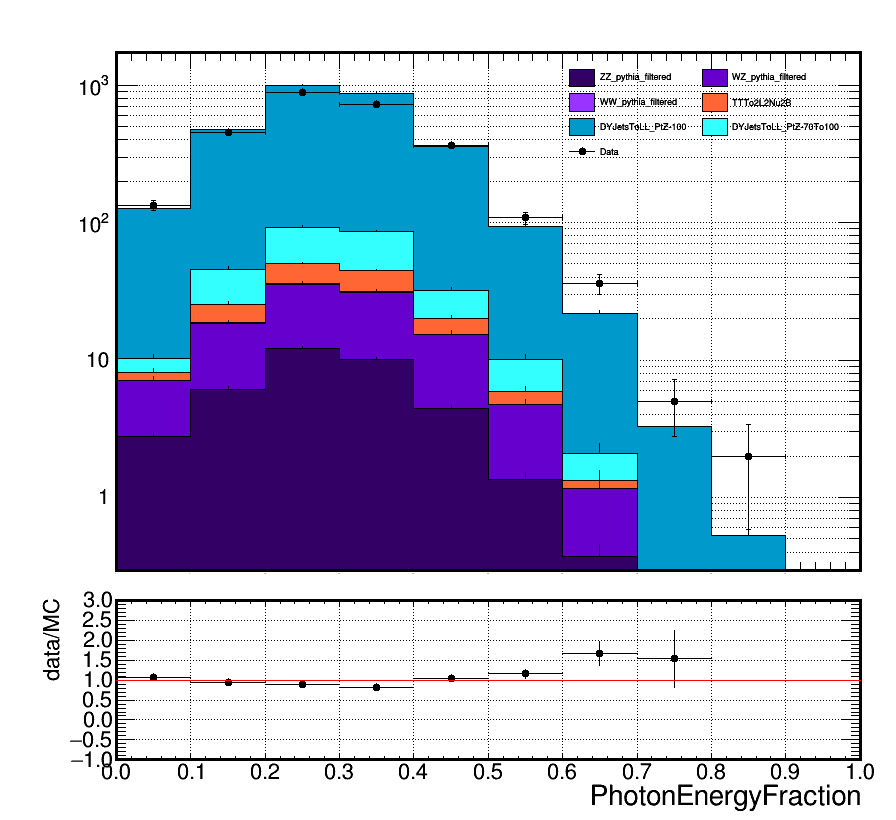
\includegraphics[scale=0.22]{figure/CH3/JetID/h_CA8jetPhoEF.png}}
  \caption{\label{fig:MuPhoEF}Comparison between data and all background samples for two jet variables. The definition of muon/photon  energy fraction is muon/photon energy divided by jet energy.}
\end{figure}

\begin{figure}[hbtp]
  \centering
  \subfigure[Charged electromagnetic energy fraction]{
    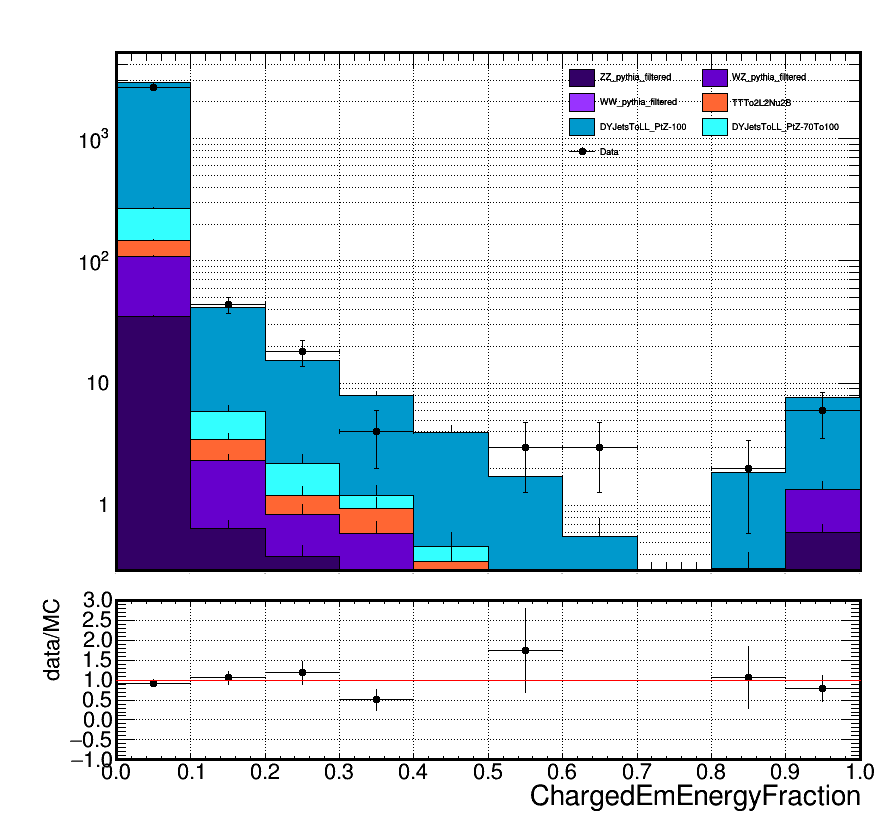
\includegraphics[scale=0.22]{figure/CH3/JetID/h_CA8jetCEmEF.png}}
  \hspace{0.5cm}
  \subfigure[Charged hadron energy fraction]{
    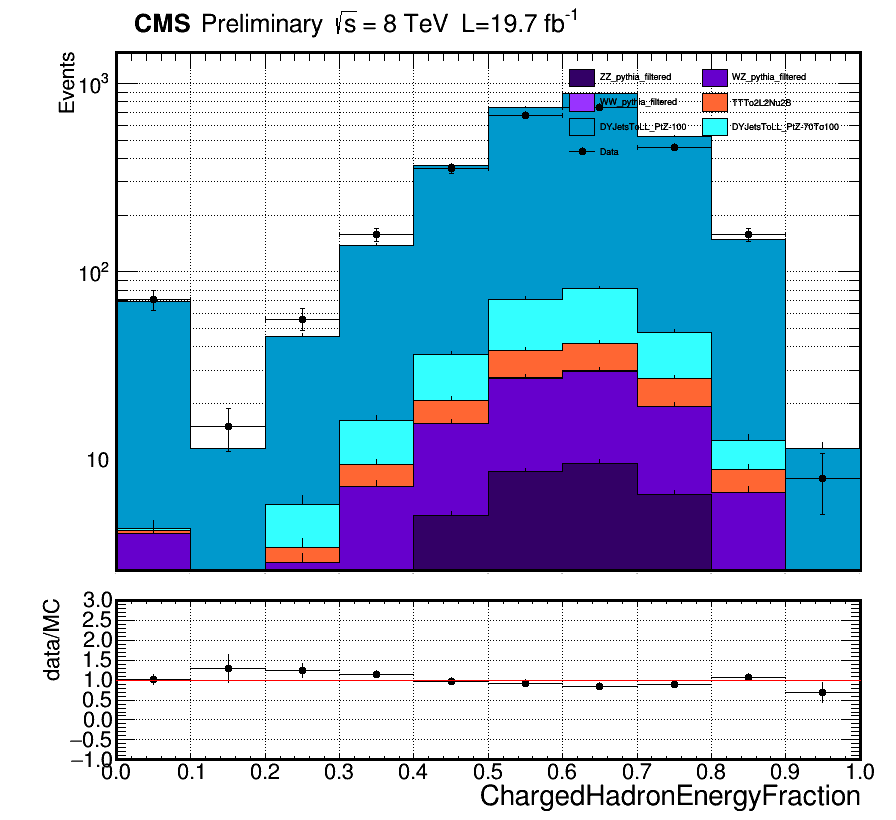
\includegraphics[scale=0.22]{figure/CH3/JetID/h_CA8jetCHadEF.png}}
  \caption{\label{fig:ChargedEF}Charged electromagnetic/hadron energy fraction is defined by the ratio of the energy of charged particles in ECAL/HCAL to the jet energy.}
\end{figure}

\begin{figure}[hbtp]
  \centering
  \subfigure[Neutral electromagnetic energy fraction]{
    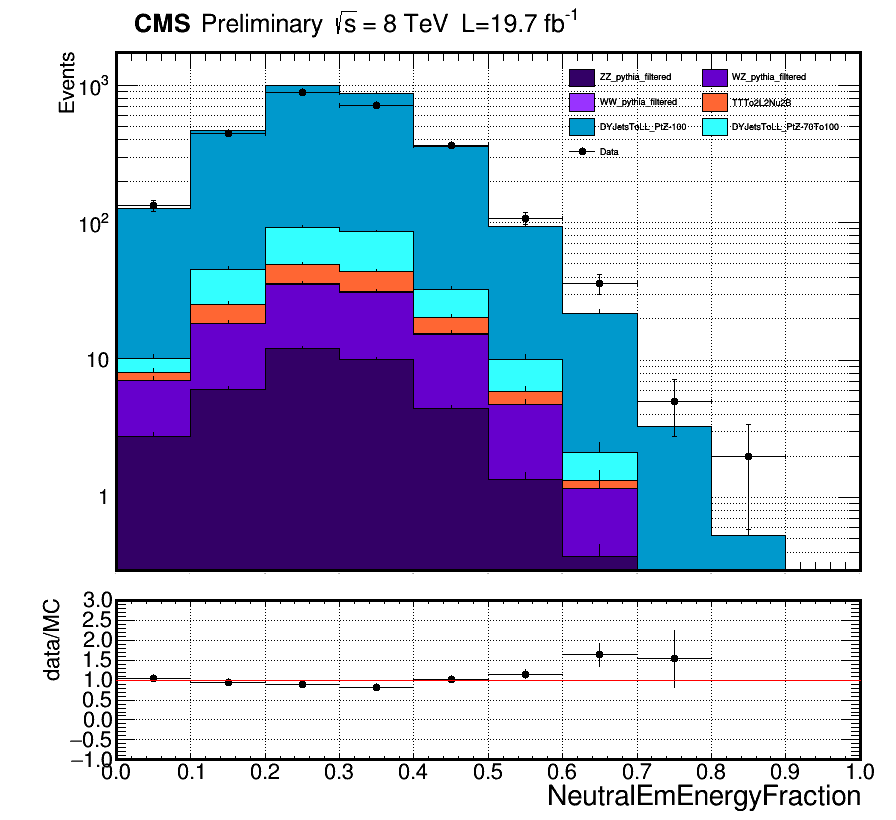
\includegraphics[scale=0.22]{figure/CH3/JetID/h_CA8jetNEmEF.png}}
  \hspace{0.5cm}
  \subfigure[Neutral hadron energy fraction]{
    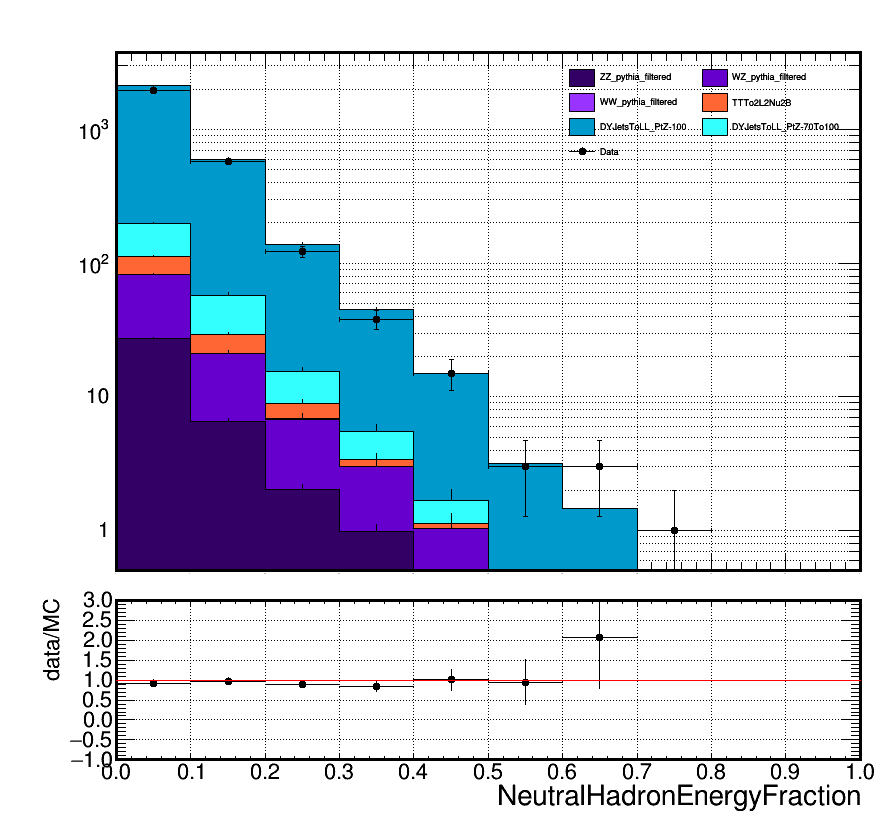
\includegraphics[scale=0.22]{figure/CH3/JetID/h_CA8jetNHadEF.png}}
  \caption{\label{fig:NeutralEF}Neutral electromagnetic/hadron energy fraction is defined by the ratio of the energy of neutral particles in ECAL/HCAL to the jet energy.}
\end{figure}

\begin{figure}[hbtp]
  \centering
  \subfigure[Jet multiplicity]{
    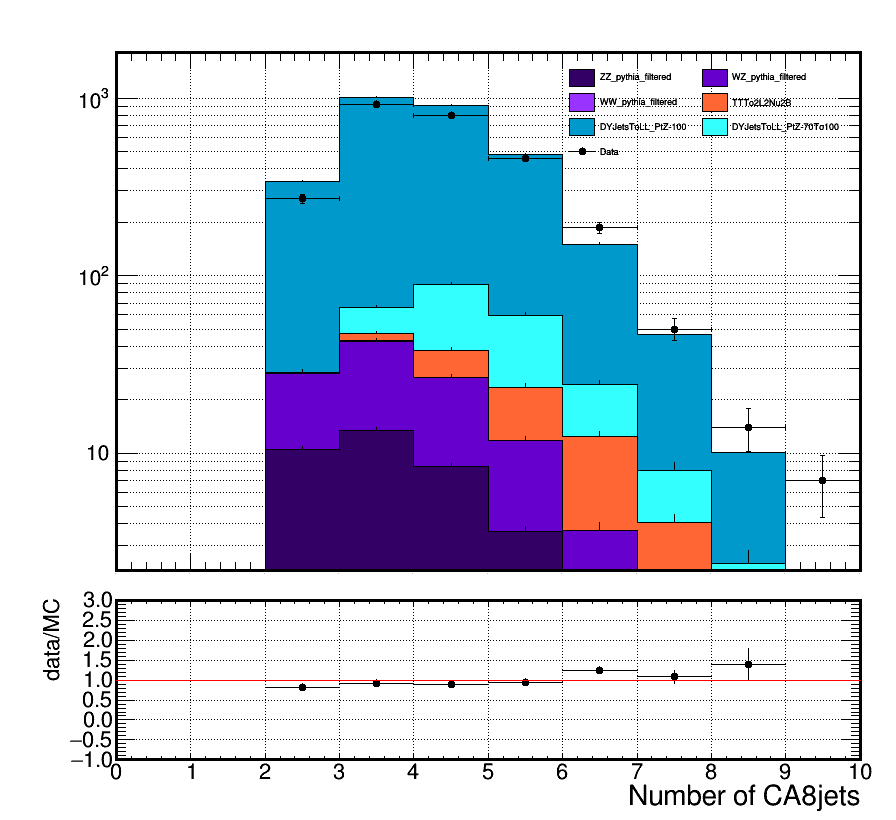
\includegraphics[scale=0.22]{figure/CH3/Jet_kinematics/h_nCA8jet.png}}
  \hspace{0.5cm}
  \subfigure[CA8jet $p_{T}$]{
    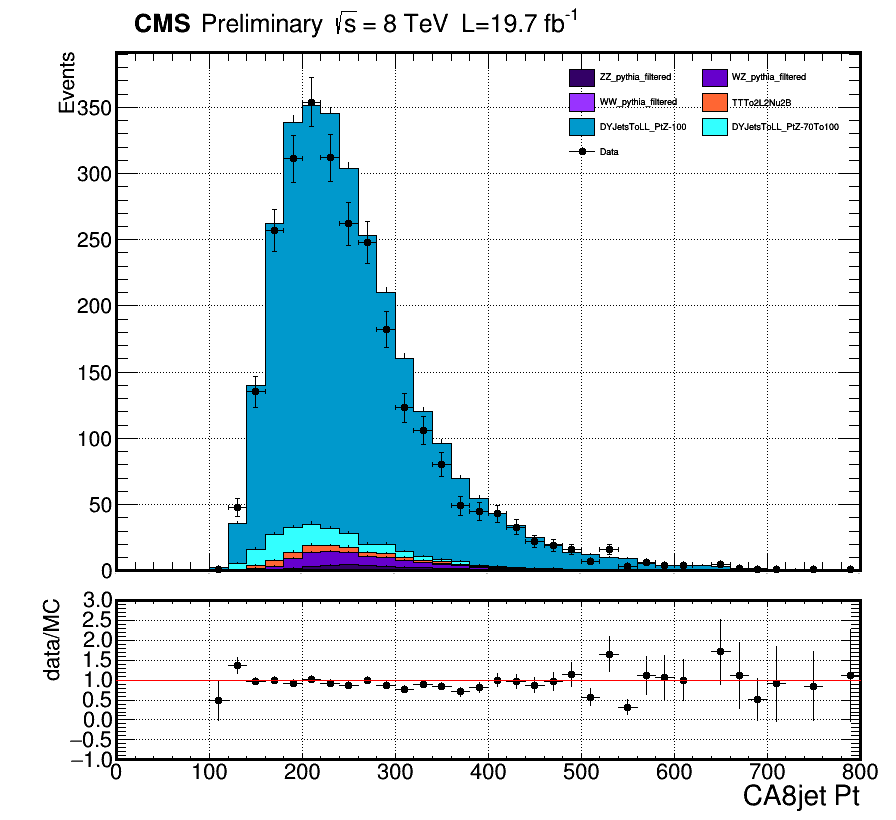
\includegraphics[scale=0.22]{figure/CH3/Jet_kinematics/h_CA8jetPt.png}}
  \caption{\label{fig:nCA8jetPt}Comparison between data and MC in SB region using jet multiplicity (number of jets) and CA8jet transverse momentum.}
\end{figure}

\begin{figure}[hbtp]
  \centering
  \subfigure[CA8jet $\eta$]{
    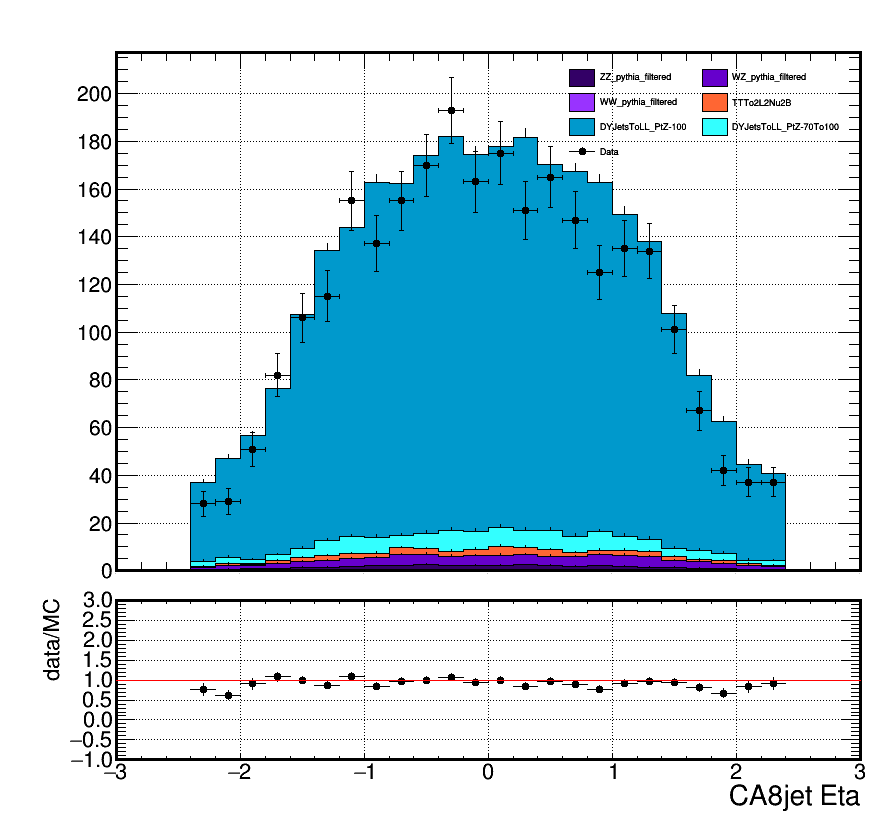
\includegraphics[scale=0.22]{figure/CH3/Jet_kinematics/h_CA8jetEta.png}}
  \hspace{0.5cm}
  \subfigure[CA8jet $\phi$]{
    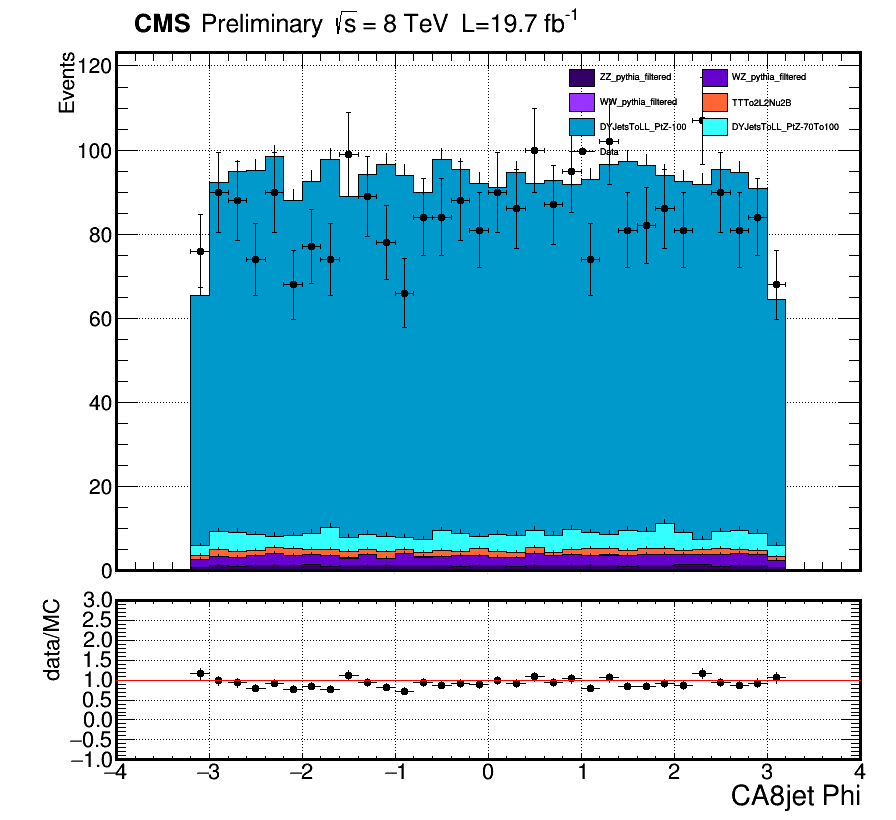
\includegraphics[scale=0.22]{figure/CH3/Jet_kinematics/h_CA8jetPhi.png}}
  \caption{\label{fig:CA8jetEtaPhi}Comparison between data and MC in SB region using CA8jet $\eta$ and $\phi$.}
\end{figure}

\begin{figure}[hbtp]
  \centering
  \subfigure[Prunedjet mass]{
    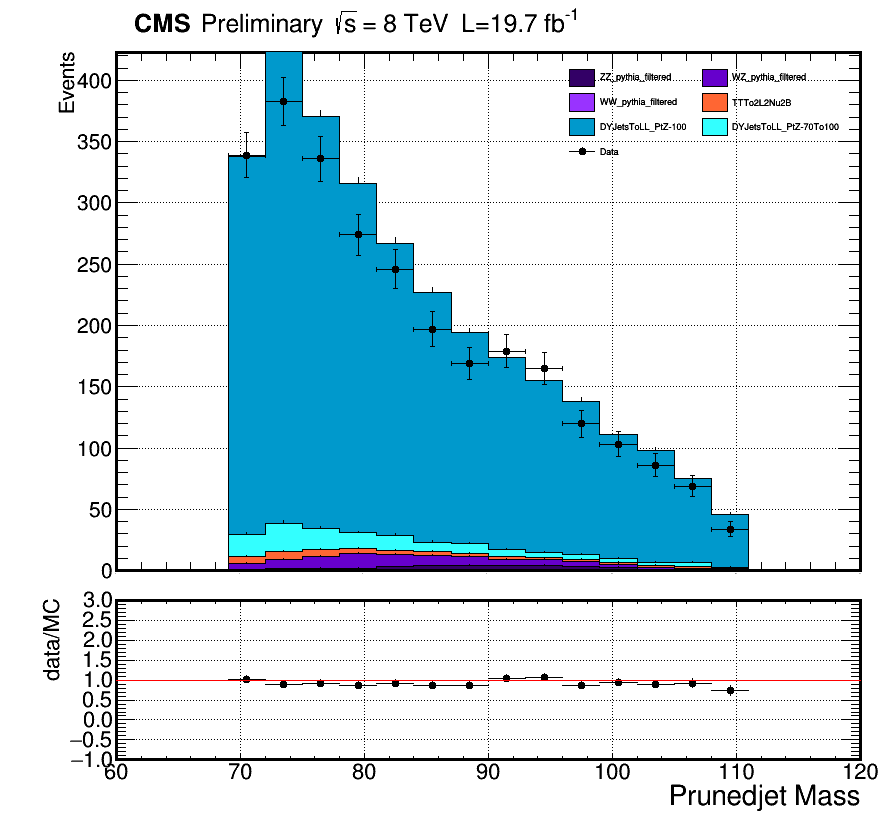
\includegraphics[scale=0.22]{figure/CH3/Jet_kinematics/h_PrunedjetM.png}}
  \hspace{0.5cm}
  \subfigure[$\Delta R$ between two subjets]{
    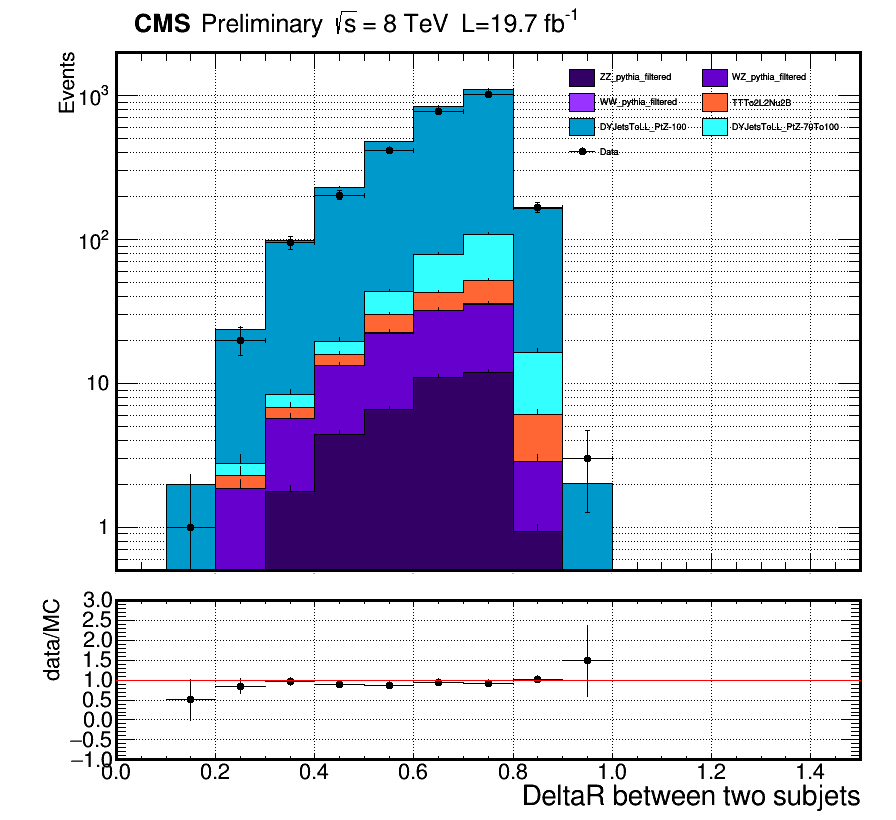
\includegraphics[scale=0.22]{figure/CH3/Jet_kinematics/h_DeltaRjj.png}}
  \caption{\label{fig:prunedmassDRjj}Left: the prunedjet mass in the SB region. Right: the spatial distance between two subjets within the CA8jet.}
\end{figure}

\begin{figure}[hbtp]
  \centering
  \subfigure[Z mass]{
    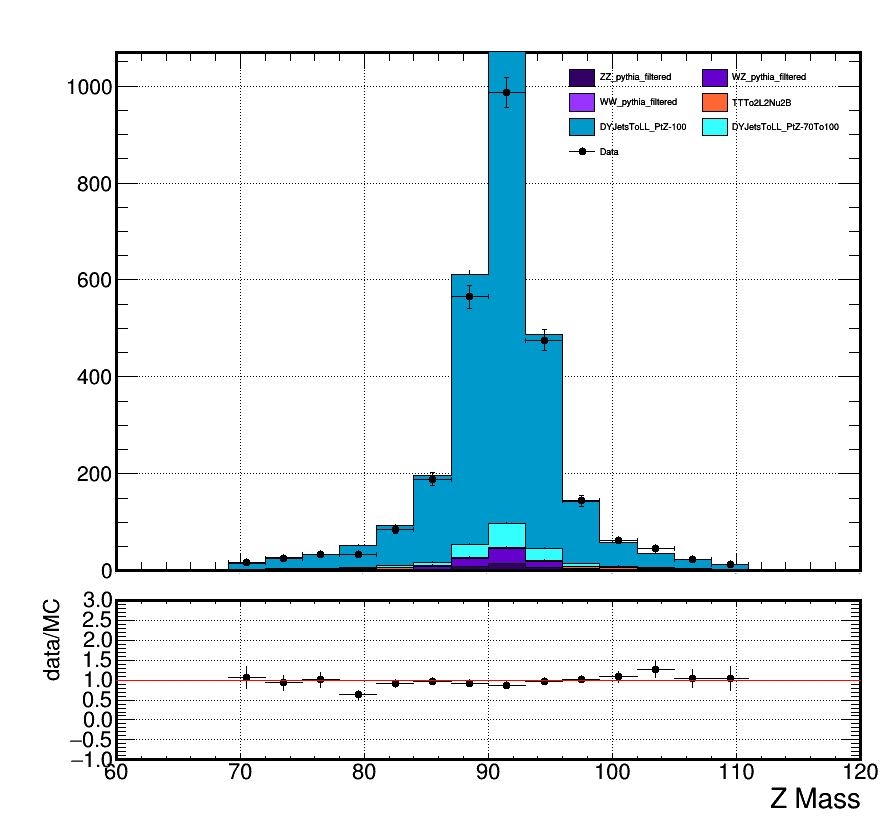
\includegraphics[scale=0.22]{figure/CH3/Z_kinematics/h_ZMass.png}}
  \hspace{0.5cm}
  \subfigure[Z $p_{T}$]{
    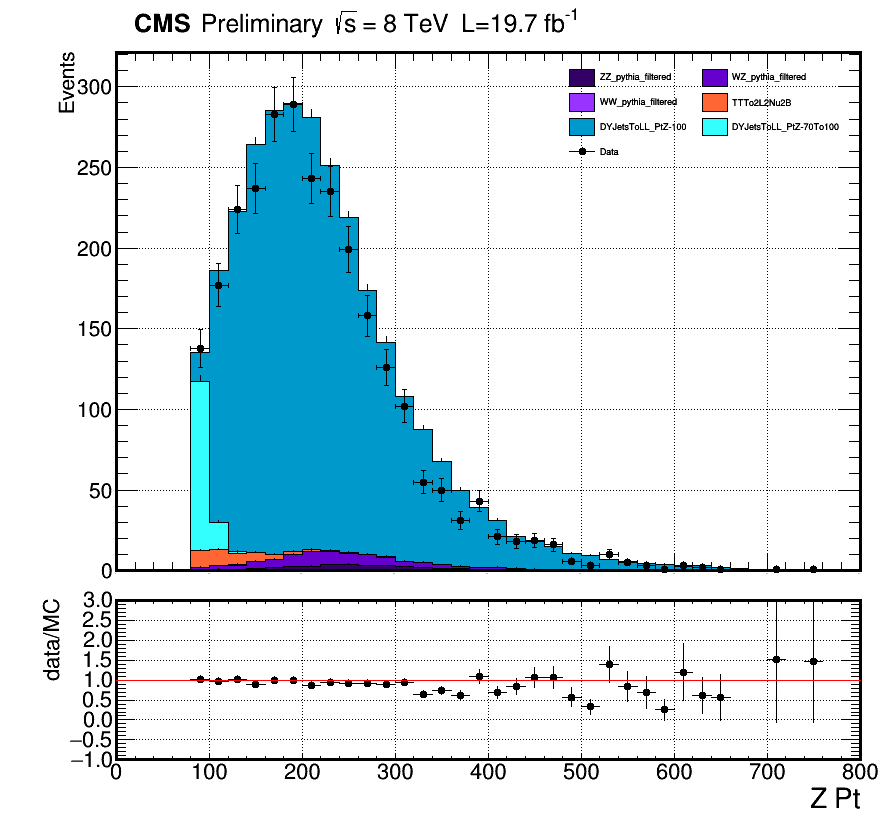
\includegraphics[scale=0.22]{figure/CH3/Z_kinematics/h_ZPt.png}}
  \caption{\label{fig:ZMassPt}Comparison between data and MC in SB region using mass and transverse momentum of reconstructed Z boson.}
\end{figure}

\begin{figure}[hbtp]
  \centering
  \subfigure[Z $\eta$]{
    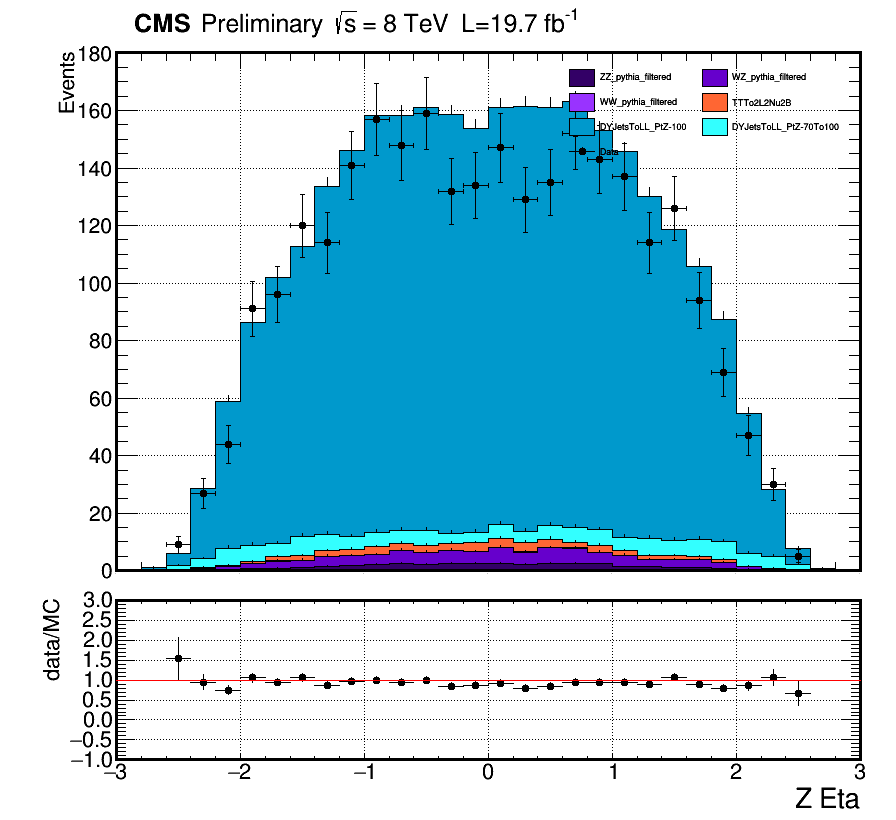
\includegraphics[scale=0.22]{figure/CH3/Z_kinematics/h_ZEta.png}}
  \hspace{0.5cm}
  \subfigure[Z $\phi$]{
    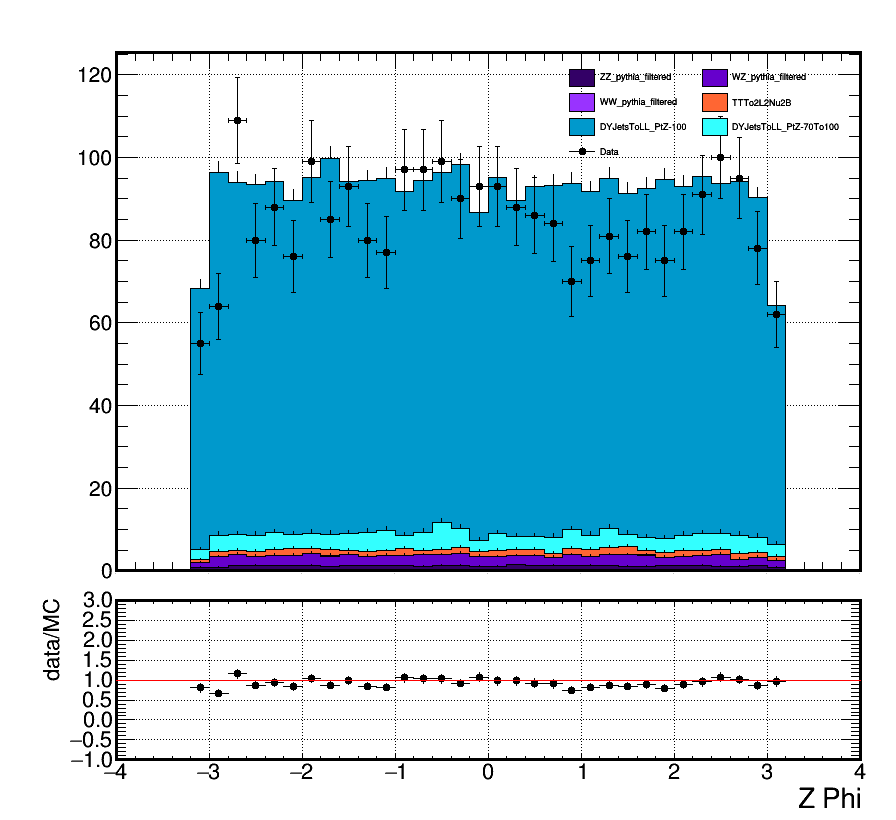
\includegraphics[scale=0.22]{figure/CH3/Z_kinematics/h_ZPhi.png}}
  \caption{\label{fig:ZEtaPhi}Comparison between data and MC in SB region using $\eta$ and $\phi$ of reconstructed Z boson.}
\end{figure}

\begin{figure}[hbtp]
  \begin{center}
    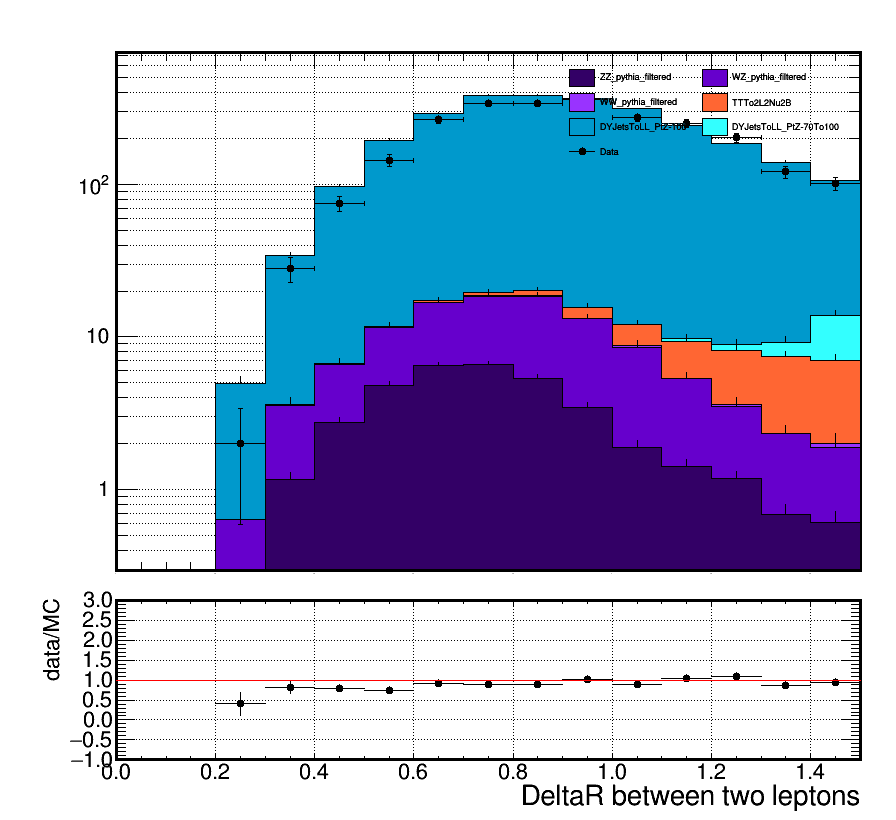
\includegraphics[width=0.5\textwidth]{figure/CH3/Z_kinematics/h_DeltaRll.png}
  \end{center}
  \caption{\label{fig:DeltaRll}$\Delta R$ between the two selected leptons.}
\end{figure}

\newpage
\section{Background Estimation}

The final aim of this analysis is to test the $Z'$ hypothesis with the observed data, it is important to elaborate a trustworthy strategy for the SM background estimation. Despite the good description of the event kinematics provided by the MC simulation, it is more advisable to minimize the dependence on the MC and develop a data driven strategy.

\subsection{$\alpha$ ratio method}

$\alpha$ ratio is a data driven method in order to estimate the final background in data signal region. We consider the $m_{Zh}$ MC mass spectrum in the SR and SB, then a ratio $\alpha$($m_{Zh}$) of the two is created. This factor $\alpha$ allows prediction of the mass spectrum in the signal region starting from the observed distribution in the sidebands. Under the assumption that this estrapolation from the sidebands to the signal region works in the same way both for data and MC, we can estimate the final background distribution in data signal region by multipling the $m_{Zh}$ mass spectrum observed in the sidebands by this $\alpha$ ratio:

\begin{align}
  \label{eq:AlphaRatio}
  N_{SR}^{data}(m_{Zh}) = N_{SB}^{data}(m_{Zh})\times \frac{N^{MC}_{SR}(m_{Zh})}{N^{MC}_{SB}(m_{Zh})}\equiv N_{SB}^{data}(m_{Zh})\times \alpha (m_{Zh})
\end{align}

We divided the spectrum in 14 non-uniform width bins, as shown in Table~\ref{tab:bin}, accordingly to the decreasing statistics in the high mass tail.

\begin{center}
  \begin{table}[h]
    \begin{center}
      \begin{tabular}{c|c}
        \hline
        \bf Bin & \bf GeV \\
        \hline
        \hline
        1 & [680, 720] \\
        2 & [720, 760] \\
        3 & [760, 800] \\
        4 & [800, 840] \\
        5 & [840, 920] \\
        6 & [920, 1000] \\
        7 & [1000, 1100] \\
        8 & [1100, 1250] \\
        9 & [1250, 1400] \\
        10 & [1400, 1600] \\
        11 & [1600, 1800] \\
        12 & [1800, 2000] \\
        13 & [2000, 2200] \\
        14 & [2200, 2400] \\
        \hline
      \end{tabular}
    \end{center}
    \caption{\label{tab:bin}Binning of the Zh invariant mass range.}
  \end{table}
\end{center}

Finally, we multiplied the $\alpha$ ratio to the sidebands data $m_{Zh}$ distribution and obtained the prediction number of backgrounds in data signal region.

\begin{figure}[hbtp]
  \begin{center}
    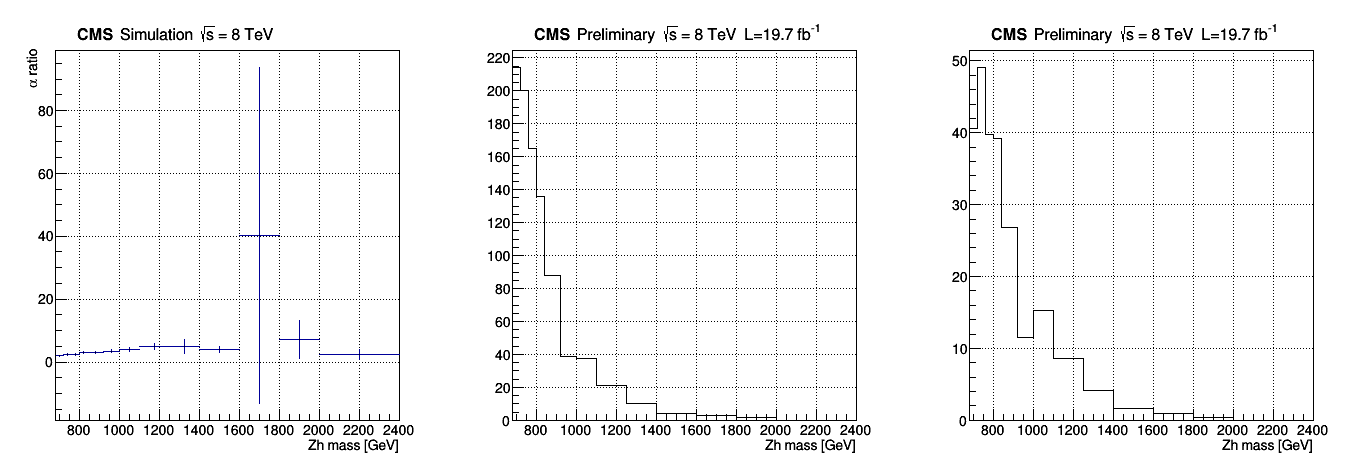
\includegraphics[width=\textwidth]{figure/CH3/alpha_new.png}
  \end{center}
  \caption{\label{fig:alpha}Left figure: the $\alpha$ ratio from MC simulation. Central figure: the $m_{Zh}$ distribution observed from data SB. Right figure: the predicted $m_{Zh}$ distribution in data signal region. The $m_{Zh}$ histograms are normalized to the first bin width.}
\end{figure}

\section{Signal Yields}
Since all selections have been settled, we can look at the data in the signal region now. In this section, signal efficiency and distributions of variables in SR will be reported. 

\subsection{signal efficiency}
The signal efficiency is defined by the fraction of the number of events passing final selection and the number of generated events in the signal MC samples (Table.~\ref{tab:TableSignalMC}). 

\begin{align}
  \label{eq:SIGeff}
  \epsilon_{SIG}\equiv \frac{\textup{Number of events passing the final selections}}{\textup{Number of generated events}}
\end{align}

The result of efficiencies are shown in Fig.~\ref{fig:SIG_eff_spectrum} (a). The figure shows a drop of efficiency in muon channel after signal mass of 1100 GeV, which comes from the muon isolation selection. It suggests the defect of the isolation definition. The isolation definition and its efficiency will be improved in the 13 TeV analysis.

\begin{figure}[hbtp]
  \centering
  \subfigure[Signal effciencies for each $Z'$ samples]{
    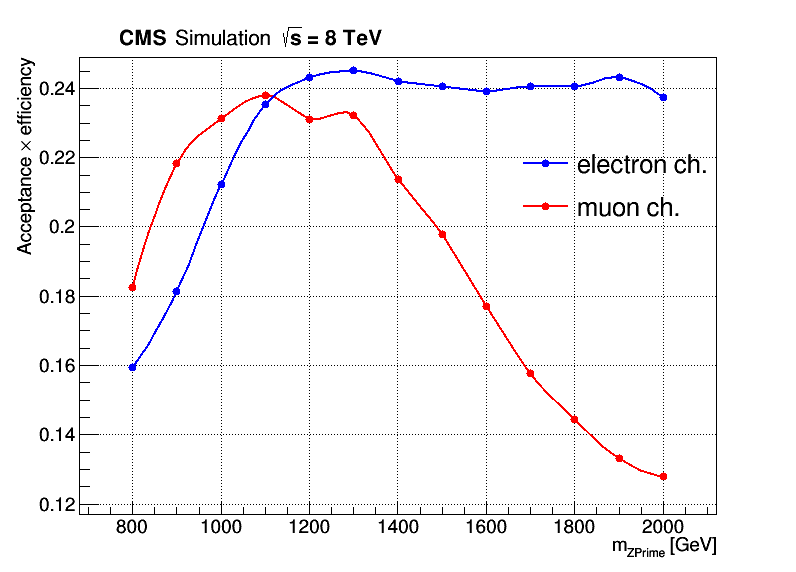
\includegraphics[scale=0.35]{figure/CH3/SIGeff.png}}
  \hspace{0.5cm}
  \subfigure[$m_{Zh}$ spectrum]{
    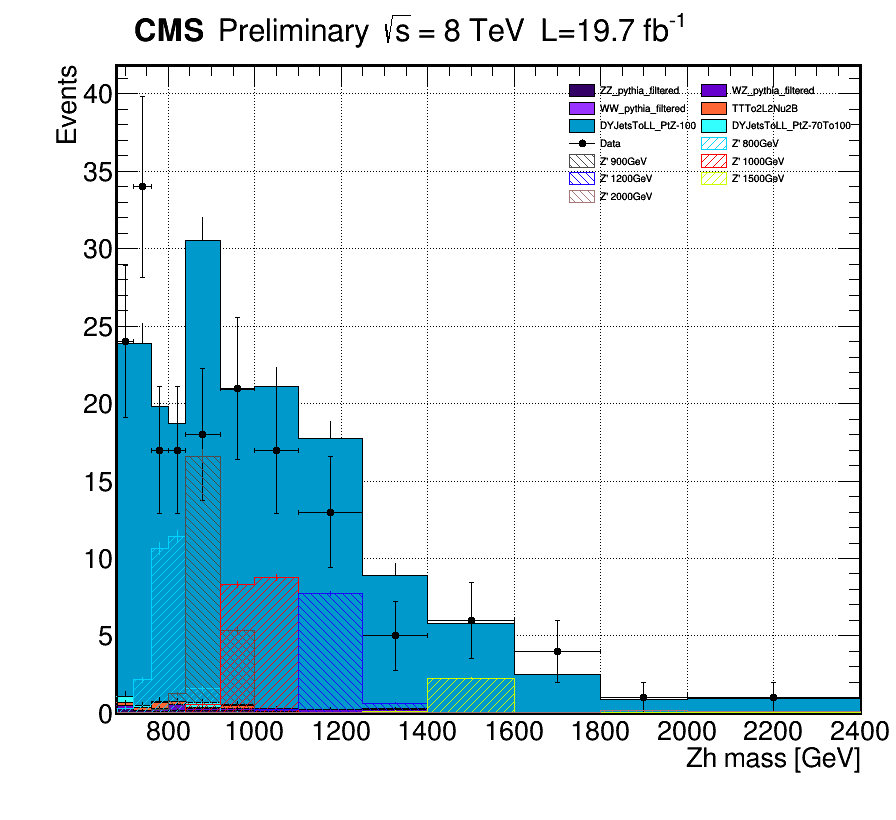
\includegraphics[scale=0.22]{figure/CH3/h_sigXMass.png}}
  \subfigure[$m_{Zh}$ spectrum (normalized bin width)]{
    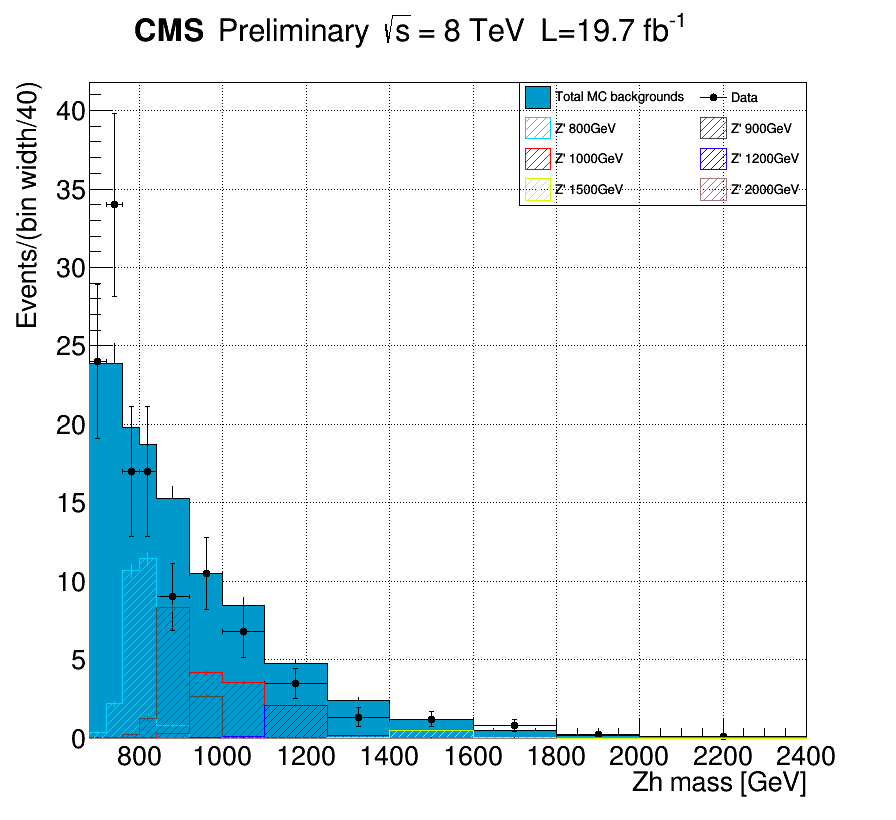
\includegraphics[scale=0.22]{figure/CH3/h_sigXMass_new.png}}
  \caption{\label{fig:SIG_eff_spectrum}(a) The signal efficiencies plot of each $Z'$ mass point. (b) Invariant mass distribution of the MC background simulation compared to the observed data and MC signal shape in the SR. (c) Normalized bin width $m_{Zh}$ distribution (bin width/bin width of the first bin).}
\end{figure}

\subsection{The $m_{Zh}$ spectrum}
The $Z'$ is reconstructed by combining the four-momentum of selected Z boson and leading jet. A comparison between data and MC of the reconstructed Zh invariant mass distribution in the signal region is shown in Fig.~\ref{fig:SIG_eff_spectrum} (b)(c). Inspecting the SR mass distributions, one can see that data do not present any significant excess from the MC expectation, so we decide to put limits on the production cross section times the branching ratio for the $Z' \rightarrow Zh$ process. This Zh invariant mass spectrum will be used for computing the limit as shape information. Furthermore, in the last chapter, the number of events in the signal yields will be used for cut and count method to set the limits.

\newpage
\subsection{The CSV distribution}
Despite the reconstructed Zh mass as shape information, we introduced another powerful variable to discriminate signal from background. The overall branching ratio for a SM Higgs decaying into $b\bar{b}$ is about 56\% and for Higgs decaying into two quarks only, the BR($h\rightarrow b\bar{b}$) is about 95\% \cite{HiggsBR}. Therefore, the b-tagging CSV working point is a power tool for searching this channel.

Although the recommend CSV selection (loose working point) from BTV group\cite{BTV-13-001} for the boosted Higgs decay result in very low effiency for both background and signal MC samples. Instead of taking selection on the CSV, we use the overall distribution as another source of shape information to set the limits. The method how we retrive the CSV distribution is shown in Table.~\ref{tab:CSVsel}.

\begin{center}
  \begin{table}[h]
    \begin{center}
      \begin{tabular}{|c|c|c|}
        \hline
        \textbf{Category} & \textbf{BTV recommend (CSVL)} & \textbf{Modified} \\ \hline
        If $\Delta R_{subjets} > $ 0.3 & subjet CSV $>$ 0.244 & use the subjets CSV shape directly\\
        If $\Delta R_{sibjets} < $ 0.3 & CA8jet CSV $>$ 0.244 & use the CA8jet CSV shape directly\\
        \hline
      \end{tabular}
    \end{center}
    \caption{\label{tab:CSVsel}The recommend selection from BTV group for boosted Higgs decay. If the $\Delta R$ between the two subjets within CA8jet larger than 0.3, applying CSVL selection on both subjets. If $\Delta R_{subjets} < 0.3$, appliny CSVL on the CA8jet. In this analysis, we use the overall CSV distributions instead of selecting events by this variable (Modified). Note that, only leading CA8jet (the Higgs candidate) and subjets within it are considered in this strategy.}
  \end{table}
\end{center}

The comparison of the CSV distributions between simulation background, signal and data is shown in Fig.~\ref{fig:h_sigCSV}. Note that, the area of each distribution is set to one in order to compare the shape difference. Inspecting Fig.~\ref{fig:h_sigCSV}, signal shapes tend to distribute on the right side while the backgrounds tend to be on the left, which shows the discriminating power of CSV variable. We only report and use the distribution from the $\Delta R > 0.3$ category to set the final limits because of lack of statics in the CA8jet CSV case. The higher CSV score means the subjet acts more like a b-jet.

\begin{figure}[hbtp]
  \begin{center}
    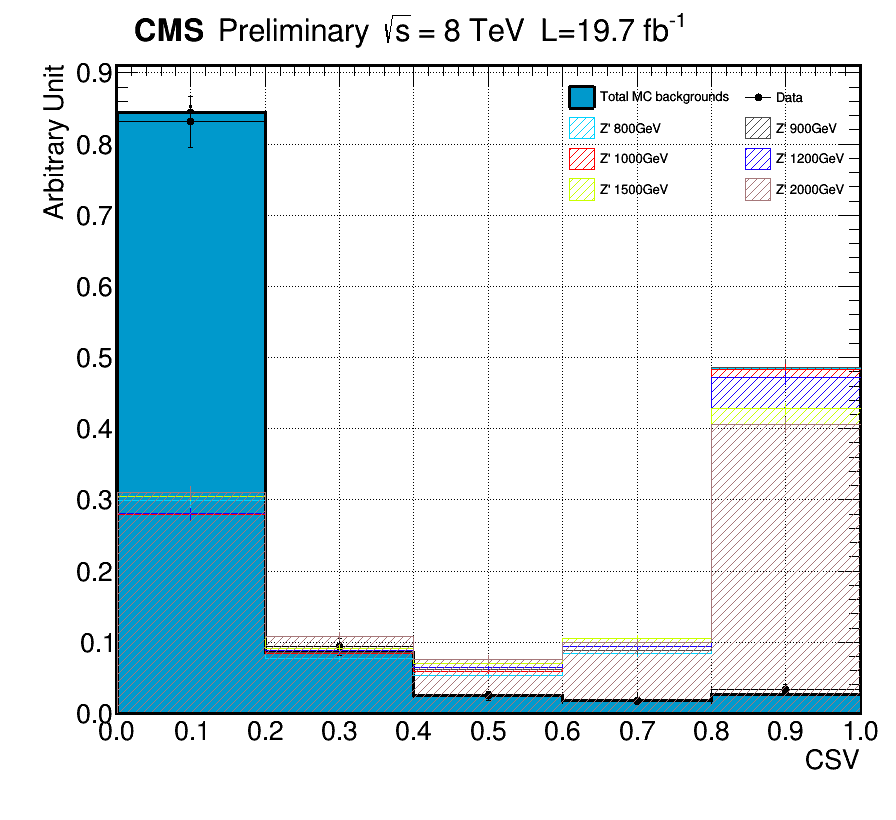
\includegraphics[width=0.5\textwidth]{figure/CH3/h_sigCSV.png}
  \end{center}
  \caption{\label{fig:h_sigCSV}The CSV distribution comparison between data and MC samples in SR.}
\end{figure}

Finally, we combine the CSV and the Zh mass distribution, making 2D histograms. Results of MC backgrounds, signal and data are shown in next pages.

\begin{figure}[hbtp]
  \centering
  \subfigure[CSV-$m_{Zh}$ distribution of total MC background]{
    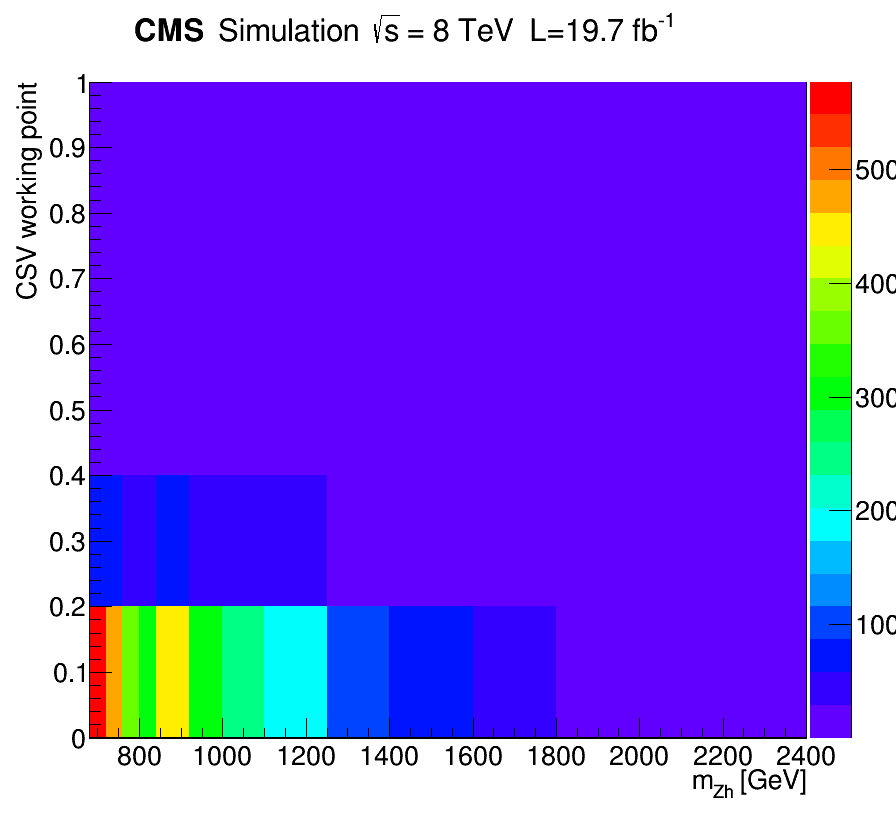
\includegraphics[scale=0.22]{figure/CH3/h2_bkgCSV}}
  \hspace{0.5cm}
  \subfigure[CSV-$m_{Zh}$ distribution of total data]{
    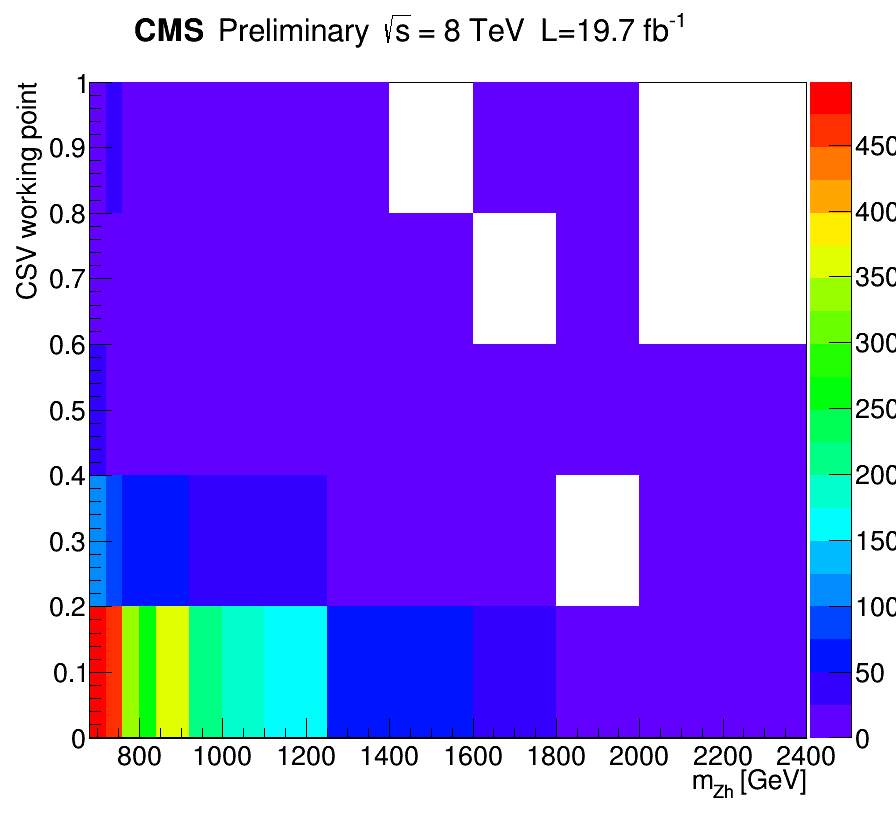
\includegraphics[scale=0.22]{figure/CH3/h2_dataCSV.png}}
  \caption{\label{fig:h2_bkg_data}The combined 2D shape result of data and MC background in SR.}
\end{figure}

\begin{figure}[hbtp]
  \centering
  \subfigure[CSV-$m_{Zh}$ distribution of 800 GeV $Z'$ mass signal sample]{
    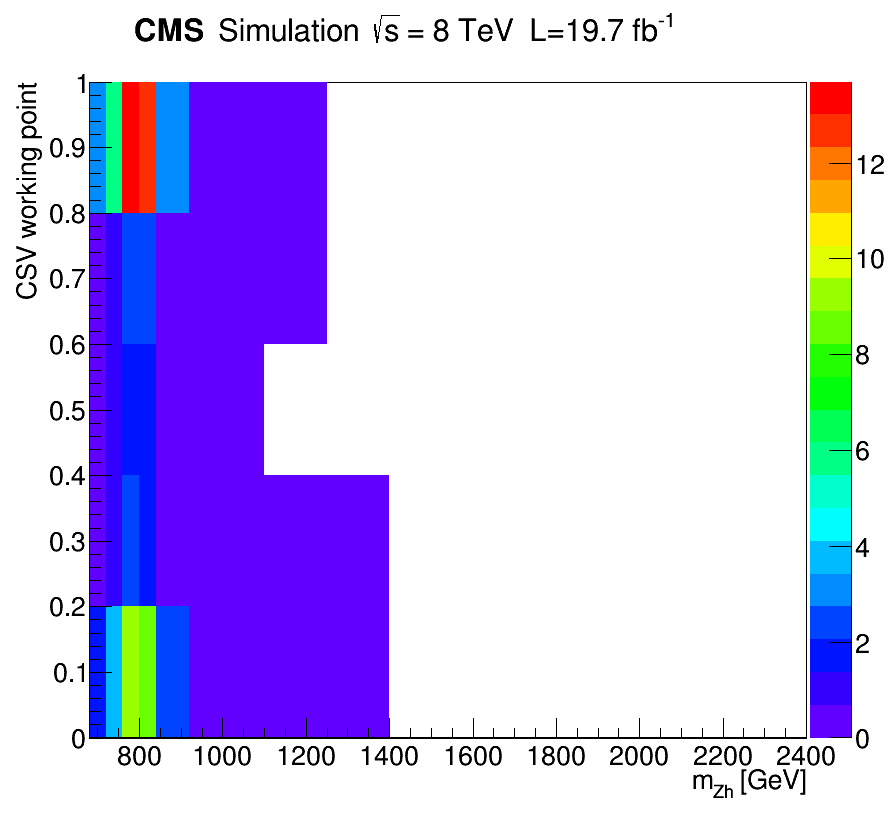
\includegraphics[scale=0.22]{figure/CH3/h2_sig800.png}}
  \hspace{0.5cm}
  \subfigure[CSV-$m_{Zh}$ distribution of 1000 GeV $Z'$ mass signal sample]{
    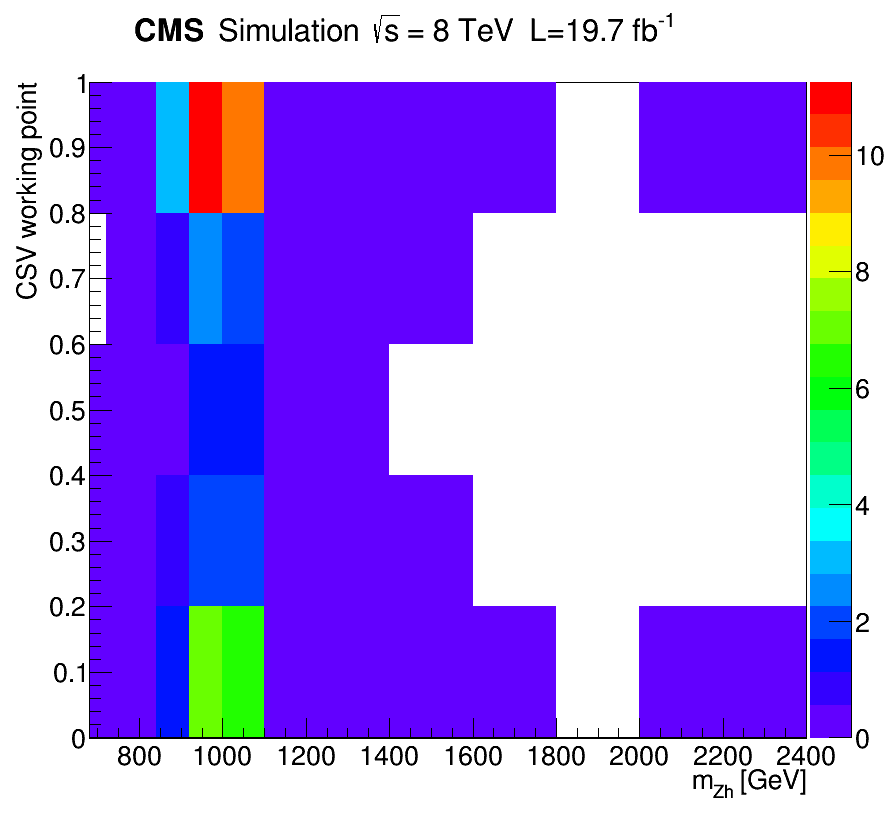
\includegraphics[scale=0.22]{figure/CH3/h2_sig1000.png}}
  \caption{\label{fig:h2_sig1}The combined 2D shape result in SR of 800 GeV and 1000 GeV signal MC samples.}
\end{figure}

\begin{figure}[hbtp]
  \centering
  \subfigure[CSV-$m_{Zh}$ distribution of 1500 GeV $Z'$ mass signal sample]{
    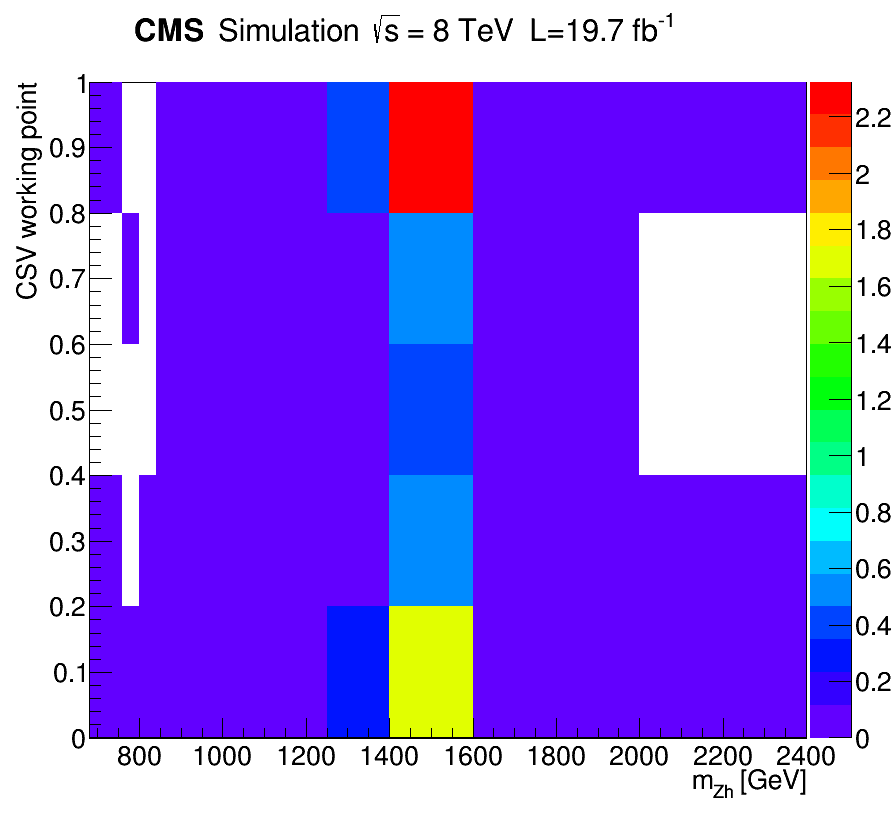
\includegraphics[scale=0.22]{figure/CH3/h2_sig1500.png}}
  \hspace{0.5cm}
  \subfigure[CSV-$m_{Zh}$ distribution of 2000 GeV $Z'$ mass signal sample]{
    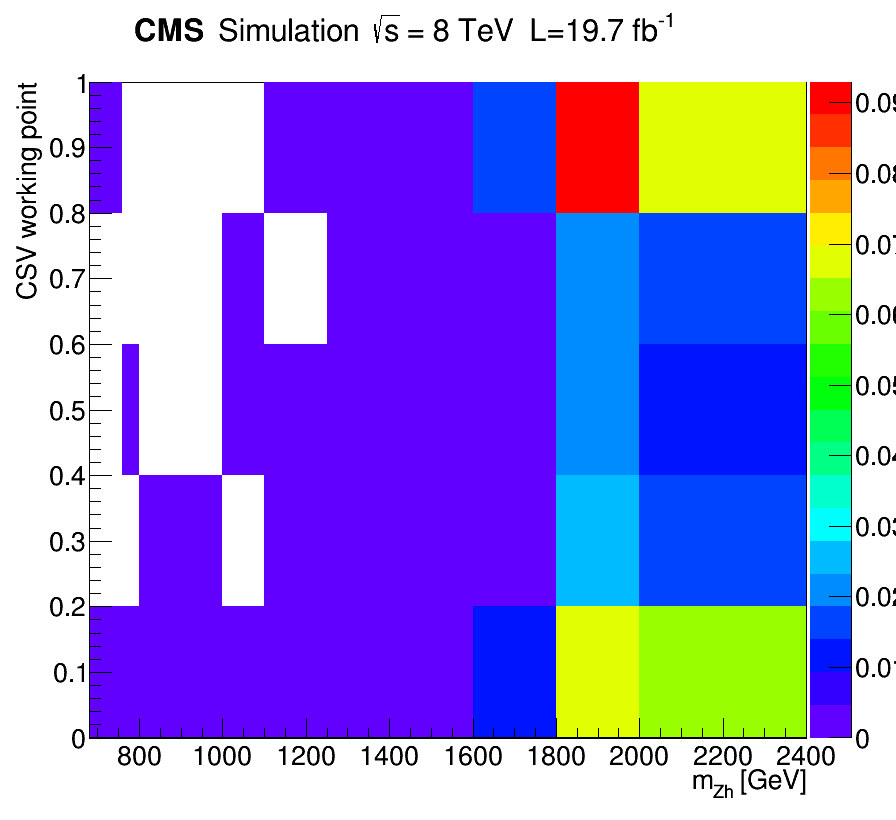
\includegraphics[scale=0.22]{figure/CH3/h2_sig2000.png}}
  \caption{\label{fig:h2_sig2}The combined 2D shape result in SR of 1500 GeV and 2000 GeV signal MC samples.}
\end{figure}


